\lab{Advanced Numpy}{Advanced Numpy}
\label{lab:AdvancedNumpy}
\objective{NumPy is a vast library with many useful functions that can be easily forgotten if not used and reviewed. This lab will help you remember some of its functionality that you may have forgotten and give you a few new functions to master.}

\begin{info}
Some of this lab is review, but there is new material near the end and additional materials beyond that.
\end{info}

\section*{Data Access} % ======================================================

\subsection*{Array Slicing} % -------------------------------------------------

Indexing for a 1-D NumPy array uses the slicing syntax \li{x[start:stop:step]}.
If there is no colon, a single entry of that dimension is accessed.
With a colon, a range of values is accessed.
For multi-dimensional arrays, use a comma to separate slicing syntax for each axis.

\begin{lstlisting}
# Make an array of the integers from 0 to 10 (exclusive).
>>> x = np.arange(10)
>>> x
array([0, 1, 2, 3, 4, 5, 6, 7, 8, 9])

# Access elements of the array with slicing syntax.
>>> x[3]                            # The element at index 3.
3
>>> x[:3]                           # Everything up to index 3 (exclusive).
array([0, 1, 2])
>>> x[3:]                           # Everything from index 3 on.
array([3, 4, 5, 6, 7, 8, 9])
>>> x[3:8]                          # The elements from index 3 to 8.
array([3, 4, 5, 6, 7])

>>> A = np.array([[0,1,2,3,4],[5,6,7,8,9]])
>>> A
array([[0, 1, 2, 3, 4],
       [5, 6, 7, 8, 9]])

# Use a comma to separate the dimensions for multi-dimensional arrays.
>>> A[1, 2]                         # The element at row 1, column 2.
7
>>> A[:, 2:]                        # All of the rows, from column 2 on.
array([[2, 3, 4],
       [7, 8, 9]])
\end{lstlisting}

% See Appendix \ref{appendix:numpy-visual-guide} for visual examples of slicing.

\begin{info} % Views vs. Copies.
Indexing and slicing operations return a \emph{view} of the array.
Changing a view of an array also changes the original array.
In other words, \textbf{arrays are mutable}.
To create a copy of an array, use \li{np.copy()} or the array's \li{copy()} method.
Changes to a copy of an array does not affect the original array, but copying an array uses more time and memory than getting a view.
\end{info}

\subsection*{Fancy Indexing} % ------------------------------------------------

So-called \emph{fancy indexing} is a second way to access or change the elements of an array.
Instead of using slicing syntax, provide either an array of indices or an array of boolean values (called a \emph{mask}) to extract specific elements.

\begin{lstlisting}
>>> x = np.arange(0, 50, 10)        # The integers from 0 to 50 by tens.
>>> x
array([ 0, 10, 20, 30, 40])

# An array of integers extracts the entries of 'x' at the given indices.
>>> index = np.array([3, 1, 4])     # Get the 3rd, 1st, and 4th elements.
>>> x[index]                        # Same as np.array([x[i] for i in index]).
array([30, 10, 40])

# A boolean array extracts the elements of 'x' at the same places as 'True'.
>>> mask = np.array([True, False, False, True, False])
>>> x[mask]                         # Get the 0th and 3rd entries.
array([ 0, 30])
\end{lstlisting}

Fancy indexing is especially useful for extracting or changing the values of an array that meet some sort of criterion.
Use comparison operators like \li{<} and \li{==} to create masks.

\begin{lstlisting}
>>> y = np.arange(10, 20, 2)        # Every other integers from 10 to 20.
>>> y
array([10, 12, 14, 16, 18])

# Extract the values of 'y' larger than 15.
>>> mask = y > 15                   # Same as np.array([i > 15 for i in y]).
>>> mask
<<array([False, False, False,  True,  True], dtype=bool)>>
>>> y[mask]                         # Same as y[y > 15]
array([16, 18])

# Change the values of 'y' that are larger than 15 to 100.
>>> y[mask] = 100
>>> print(y)
[10 12 14  100  100]
\end{lstlisting}

While indexing and slicing always return a view, fancy indexing always returns a copy.

\begin{problem} % Slicing / Fancy Indexing
Write a function that accepts a single array as input.
Make a copy of the array, then use fancy indexing to set all negative entries of the copy to $0$.
Return the resulting array.
\end{problem}

\section*{Array Manipulation} % ===============================================

\subsection*{Shaping} % -------------------------------------------------------

An array's \li{shape} attribute describes its dimensions.
Use \li{np.reshape()} or the array's \li{reshape()} method to give an array a new shape.
The total number of entries in the old array and the new array must be the same in order for the shaping to work correctly.
Using a \li{-1} in the new shape tuple makes the specified dimension as long as necessary.
% Whenever possible, \li{np.reshape()} returns a view.

\begin{lstlisting}
>>> A = np.arange(12)               # The integers from 0 to 12 (exclusive).
>>> print(A)
[ 0  1  2  3  4  5  6  7  8  9 10 11]

# 'A' has 12 entries, so it can be reshaped into a 3x4 matrix.
>>> A.reshape((3,4))                # The new shape is specified as a tuple.
array([[ 0,  1,  2,  3],
       [ 4,  5,  6,  7],
       [ 8,  9, 10, 11]])

# Reshape 'A' into an array with 2 rows and the appropriate number of columns.
>>> A.reshape((2,-1))
array([[ 0,  1,  2,  3,  4,  5],
       [ 6,  7,  8,  9, 10, 11]])
\end{lstlisting}

Use \li{np.ravel()} to flatten a multi-dimensional array into a 1-D array and \li{np.transpose()} or the \li{T} attribute to transpose a 2-D array in the matrix sense.

\begin{lstlisting}
>>> A = np.arange(12).reshape((3,4))
>>> A
array([[ 0,  1,  2,  3],
       [ 4,  5,  6,  7],
       [ 8,  9, 10, 11]])

# Flatten 'A' into a one-dimensional array.
>>> np.ravel(A)                     # Equivalent to A.reshape(A.size)
array([ 0,  1,  2,  3,  4,  5,  6,  7,  8,  9, 10, 11])

# Transpose the matrix 'A'.
>>> A.T                             # Equivalent to np.transpose(A).
array([[ 0,  4,  8],
       [ 1,  5,  9],
       [ 2,  6, 10],
       [ 3,  7, 11]])
\end{lstlisting}

\begin{info} % All 1-D Numpy arrays are flat!
By default, all NumPy arrays that can be represented by a single dimension, including column slices, are automatically reshaped into ``flat'' 1-D arrays.
For example, by default an array will have 10 elements instead of 10 arrays with one element each.
Though we usually represent vectors vertically in mathematical notation, NumPy methods such as \li{dot()} are implemented to purposefully work well with 1-D ``row arrays''.

\begin{lstlisting}
>>> A = np.arange(10).reshape((2,5))
>>> A
array([[0, 1, 2, 3, 4],
       [5, 6, 7, 8, 9]])

# Slicing out a column of A still produces a "flat" 1-D array.
>>> x = A[:,1]                      # All of the rows, column 1.
>>> x
array([1, 6])                       # Not array([[1],
>>> x.shape                         #            [6]])
(2,)
>>> x.ndim
1
\end{lstlisting}

However, it is occasionally necessary to change a 1-D array into a ``column array''.
Use \li{np.reshape()}, \li{np.vstack()}, or slice the array and put \li{np.newaxis} on the second axis.
Note that \li{np.transpose()} does not alter 1-D arrays.

\begin{lstlisting}
>>> x = np.arange(3)
>>> x
array([0, 1, 2])

>>> x.reshape((-1,1))               # Or x[:,np.newaxis] or np.vstack(x).
array([[0],
       [1],
       [2]])
\end{lstlisting}

Do not force a 1-D vector to be a column vector unless necessary.
\end{info}

\subsection*{Stacking} % ------------------------------------------------------

NumPy has functions for \emph{stacking} two or more arrays with similar dimensions into a single block matrix.
Each of these methods takes in a single tuple of arrays to be stacked in sequence.

\begin{table}[H]
\centering
\begin{tabular}{r|l}
    Function & Description\\
    \hline
    % % Shaping methods, already discussed
    % \li{reshape()} & Return a view of the array with a changed shape.\\
    % \li{ravel()} & Make a flattened version of an array, return a view if possible.\\
    % \li{transpose()} & Permute the dimensions of the array (also \li{ndarray.T}).\\
    % \hline
    \li{concatenate()} & Join a sequence of arrays along an existing axis\\
    \li{vstack()} & Stack arrays in sequence vertically (row wise).\\
    \li{hstack()} & Stack arrays in sequence horizontally (column wise).\\
    \li{column_stack()} & Stack 1-D or 2-D arrays horizontally (column wise) into a 2-D array.
\end{tabular}
\end{table}

\begin{lstlisting}
>>> A = np.arange(6).reshape((2,3))
>>> B = np.zeros((4,3))

# vstack() stacks arrays vertically (row-wise).
>>> np.vstack((A,B,A))
array([[ 0.,  1.,  2.],             # A
       [ 3.,  4.,  5.],
       [ 0.,  0.,  0.],             # B
       [ 0.,  0.,  0.],
       [ 0.,  0.,  0.],
       [ 0.,  0.,  0.],
       [ 0.,  1.,  2.],             # A
       [ 3.,  4.,  5.]])

>>> A = A.T
>>> B = B.T

# hstack() stacks arrays horizontally (column-wise).
>>> np.hstack((A,B,A))
array([[0., 3., 0., 0., 0., 0., 0., 3.],
       [1., 4., 0., 0., 0., 0., 1., 4.],
       [2., 5., 0., 0., 0., 0., 2., 5.]])
       # A      # B             # A

# column_stack() stacks arrays horizontally, including 1-D arrays.
>>> np.column_stack((A, np.zeros(3), np.ones(3), np.full(3, 2)))
array([[ 0.,  3.,  0.,  1.,  2.],
       [ 1.,  4.,  0.,  1.,  2.],
       [ 2.,  5.,  0.,  1.,  2.]])
\end{lstlisting}
%
See \url{http://docs.scipy.org/doc/numpy-1.10.1/reference/routines.array-manipulation.html} for more array manipulation routines and documentation.

\subsection*{Working with Dimensions}

In many scientific disciplines, arrays of more than 2 dimensions are readily utilized. 
Numpy's function are designed to work on these larger arrays but sometimes it's necessary to convert arrays to a different dimension. 
To do this we'll use \li{np.squeeze()} and \li{np.dstack}

\li{np.squeeze()} eliminates any superfluous dimensions in an array. 
These will be any dimension of value 1 when the shape attribute is called. 
It does not matter in which position the dimension is located. 
As a result of this, using \li{np.squeeze()} on several arrays of different shape can result in arrays of the same shape.

\begin{lstlisting}

# Define 3 arrays of different dimensions
>>> test0 = np.arange(9).reshape(1,3,3)
>>> test1 = np.arange(9).reshape(3,1,3)
>>> test2 = np.arange(9).reshape(3,3,1)

# but all arrays become the same after being squeezed
>>> np.squeeze(test0)
array([[ 0.,  1.,  2.],
       [ 3.,  4.,  5.],
       [ 6.,  7.,  8.]])

>>> np.squeeze(test1)
array([[ 0.,  1.,  2.],
       [ 3.,  4.,  5.],
       [ 6.,  7.,  8.]])

>>> np.squeeze(test2)
array([[ 0.,  1.,  2.],
       [ 3.,  4.,  5.],
       [ 6.,  7.,  8.]])

# even arrays with many extra dimensions reduce to the same matrix
>>> ridiculous = np.arange(9).reshape(1,1,1,1,3,3,1,1,1,1)
>>> np.squeeze(ridiculous)
array([[ 0.,  1.,  2.],
       [ 3.,  4.,  5.],
       [ 6.,  7.,  8.]])

# however arrays that have no 1 value in their shape will remain the same
>>> stoic = np.arange(20).reshape(2,2,5)
>>> print(stoic)
array([[[ 0,  1,  2,  3,  4],
        [ 5,  6,  7,  8,  9]],

       [[10, 11, 12, 13, 14],
        [15, 16, 17, 18, 19]]])

>>> print(np.squeeze(stoic))
array([[[ 0,  1,  2,  3,  4],
        [ 5,  6,  7,  8,  9]],

       [[10, 11, 12, 13, 14],
        [15, 16, 17, 18, 19]]])

\end{lstlisting} 

\li{np.dstack()}, on the other hand, performs like the other two stacking function except that it stacks on the third dimensions rather than the first or second. 
For example, using \li{np.dstack()} on two matrices of shape $(3,3)$ would make a matrix of shape $(3,3,2)$. If a matrix already has three dimensions or more, \li{np.dstack()} will only affect the third one (i.e, shapes $(3,3,2,2)$ with $(3,3,2,2)$ will create $(3,3,4,2)$)

\begin{problem}
Write a function that accepts a list of arrays, squeezes them and pads them with 0's so they are the same dimensions and then stacks them along the 3rd dimension. 
Thus, the arrays in the list can, individually, be any size and dimension. However, you may assume the arrays will all be 2-dimensional once the extra dimensions are squeezed out.

Hint: Use the various stacking commands to pad the inputted arrays appropriately with 0's so that they can easily be stacked into the three dimensional array in the end. 
Again, you may assume all arrays in the list, once squeezed, will be two dimensional arrays.
\end{problem}

\subsection*{Array Broadcasting} % --------------------------------------------

As we have seen up to this point, when two arrays have the same shape, performing a binary operation (such as addition or multiplication) between these arrays automatically performs that operation elementwise.

\begin{lstlisting}
>>> x = np.array([1,2,3])
>>> y = np.array([4,5,6])
>>> x + y
array([5, 7, 9])
\end{lstlisting}

While this is useful, there are many times in which we would like to perform a binary operation on two arrays with different shapes. 

Suppose, for example, that we would like to multiply a scalar value \li{b} (in other words, a zero-dimensional array) by every element in a 1-dimensional array \li{a}.
We could accomplish this naively using a loop:

\begin{lstlisting}
>>> a = np.array([1,2,3])
>>> b = 2.0
>>> z = np.zeros(3)
>>> for i in range(3):
...     z[i] = a[i] * b
...
>>> z
array([2., 4., 6.])
\end{lstlisting}

While this approach is intuitive, we can use \emph{array broadcasting} to accomplish this task more efficiently:

\begin{lstlisting}
>>> a = np.array([1,2,3])
>>> b = 2.0
>>> z = a * b
>>> z
array([2., 4., 6.])
\end{lstlisting}

We can think of what happened in this operation as a two step process:
\begin{enumerate}
	\item[1)] First, this operation duplicated the value of \li{b=2} into the array \li{[2, 2, 2]}, which matches the dimensions of \li{a}. 
	\item[2)] Second, the multiplication \li{a * [2, 2, 2]} was performed elementwise, giving the same result as the looping procedure we used above.
\end{enumerate}
This process is visualized in the following figure:
\footnote{This and all other diagrams in this section are taken from Numpy's documentation for array broadcasting, which can be found at \url{https://numpy.org/doc/stable/user/basics.broadcasting.html}}
\begin{figure}[H]
    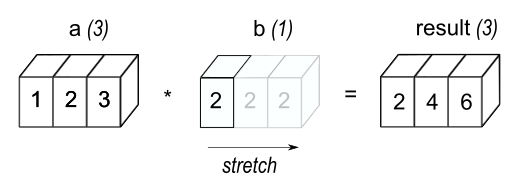
\includegraphics[width=.7\textwidth]{figures/broadcasting_scalar.png}
    \caption{Adding a scalar value to a 1-dimensional array using array broadcasting}
\end{figure}





The beauty of array broadcasting is that this duplication doesn't actually happen in memory, but the results are the same as if it had.

The exact same idea can be extended to arrays of higher dimension by using the following set of rules:

\begin{enumerate}
	\item[1)]  If the two arrays have different numbers of dimensions, add size-1 dimensions \emph{to the left} of the current dimensions of the smaller array until the number of dimensions matches.
	
	\item[2)] Stretch any singleton (size-one) dimensions in either of the two arrays to match the size of the corresponding dimension in the other array.
	
	\item[3)] Add the resulting arrays together elementwise.
\end{enumerate}

If, at any point, there are corresponding non-singleton dimensions in each array that do not match, broadcasting will raise a \li{ValueError: operands could not be broadcast together} exception.

To illustrate this concept more concretely, consider the following examples.

\begin{itemize}
	\item \textbf{Example 1}: Adding a vector to the rows of a matrix
	
	Suppose, for example, that we have a $m \times n$ array \li{a}, and we would like to add the $n$-dimensional vector \li{b} to each row of \li{a} individually. 
	
	We can list the shapes of these arrays as follows:
\begin{lstlisting}
a	(2d array):  m x n 
b	(1d array):      n
\end{lstlisting}
Step (1) of broadcasting will pad the shape of \li{b} with a size-1 dimension on the left:
\begin{lstlisting}
a	(2d array):  m x n 
b	(1d array):  1 x n
\end{lstlisting}

Notice that the leftmost dimension is a mismatch, with a 1 in \li{b}'s slot and an $m$ in \li{a}'s slot.
Thus, step (2) of the broadcasting operation will copy the inner portion of \li{b} $m$ times to match the dimension of \li{a}:
\begin{lstlisting}
a	   (2d array):  m x n 
b	   (1d array):  1 x n -> m x n
\end{lstlisting}
We can think of this operation as stacking the $n$-dimensional row vector \li{b} vertically with itself $m$ times.

Finally, step (3) of the broadcasting operation is that these two resulting arrays are added elementwise.
The result is the following:
\begin{lstlisting}
>>> a = np.array([[ 0.0,  0.0,  0.0],
...               [10.0, 10.0, 10.0],
...               [20.0, 20.0, 20.0],
...               [30.0, 30.0, 30.0]])
>>> b = np.array([1.0, 2.0, 3.0])
>>> a + b
array([[ 1.,  2.,  3.],
       [11., 12., 13.],
       [21., 22., 23.],
       [31., 32., 33.]])
\end{lstlisting}
Thus, each row of \li{a} is added to \li{b}, as desired.

A visual representation of this process is given in Figure \ref{fig:broadcasting2}:

\begin{figure}[H]
    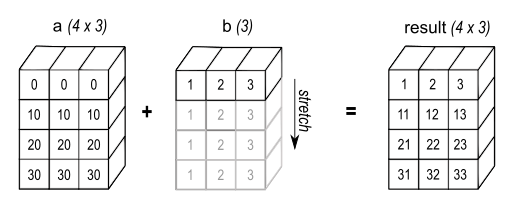
\includegraphics[width=.7\textwidth]{figures/broadcasting_vector.png}
    \caption{Adding entries of vector to the columns of a 2-dimensional array using array broadcasting}
    \label{fig:broadcasting2}
\end{figure}


\item  \textbf{Example 2}: Adding a vector to the columns of a matrix

As another example, suppose we have the same $m \times n$ array \li{a}, and we would like to add the $m$-dimensional vector \li{b} to each of its columns.

Notice that doing this in the same way as the previous example would throw an error:
\begin{lstlisting}
>>> a
array([[ 0.,  0.,  0.],
       [10., 10., 10.],
       [20., 20., 20.],
       [30., 30., 30.]])
>>> b = np.array([1., 2., 3., 4.])
>>> a + b
Traceback (most recent call last):
  File "<stdin>", line 1, in <module>
ValueError: operands could not be broadcast together with shapes (4,3) (4,)
\end{lstlisting}

To understand why this error is being thrown, notice the shapes of these two arrays after step (1) of broadcasting:
\begin{lstlisting}
a	   (2d array):  m x n 
b	   (1d array):  1 x m
\end{lstlisting}
The rightmost dimension is a mismatch, but neither dimension is $1$. This is the reason the error is thown. A visual representation of this error is given in Figure \ref{fig:broadcasting3}.

\begin{figure}[H]
    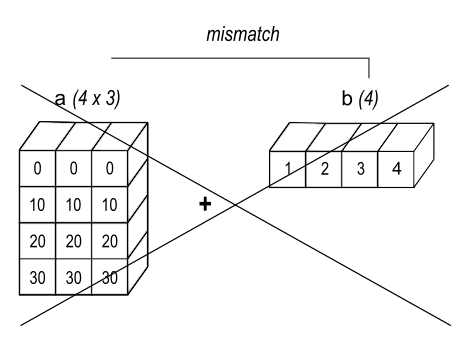
\includegraphics[width=.7\textwidth]{figures/broadcasting_mismatch.png}
    \caption{The trailing dimensions are a mismatch, so these arrays cannot be broadcast together}
    \label{fig:broadcasting3}
\end{figure}

In reality, we want to add \li{b} as a \emph{column vector}; that is, we want to make sure that the $m$'s match up in the \emph{leftmost} column. 
However, as we saw above, we can't rely on array broadcasting to do this automatically for us since it only pads with ones to the \emph{left} (thus, implicitly treating \li{b} as a row vector).

To accomplish what we want, we must explicitly reshape \li{b} to be a column vector using a \li{np.newaxis} argument (or its equivalent). 
This will pad the shape of \li{b} with a size-one dimension to the \emph{right} of its normal dimension, which will allow the dimensions to line up appropriately:
\begin{lstlisting}
a	               (2d array):  m x n 
b[:,np.newaxis]	   (1d array):  m x 1
\end{lstlisting}

The resulting operation is exactly what we want:

\begin{lstlisting}
>>> a
array([[ 0.,  0.,  0.],
       [10., 10., 10.],
       [20., 20., 20.],
       [30., 30., 30.]])
>>> b = np.array([1., 2., 3., 4.])
>>> a + b[:,np.newaxis]
array([[ 1.,  1.,  1.],
       [12., 12., 12.],
       [23., 23., 23.],
       [34., 34., 34.]])
\end{lstlisting}



\item  \textbf{Example 3}: Outer Sum of Two Vectors 

The outer sum of two vectors $\mathbf{a} \in \mathbb{R}^n, \mathbf{b} \in \mathbb{R}^m$ is defined be the matrix $A \in M_{n \times m}(\mathbb{R})$ such that 
\begin{align*}
	[A]_{ij} = a_i + b_j, \quad 1 \leq i \leq n, 1 \leq j \leq m
\end{align*} 
We can define this operation by thinking of wanting to make $m$ copies of $\mathbf{a}$ (horizontally stacked as column vectors), and add it to $n$ copies of $\mathbf{b}$ (horizontally stacked as row vectors).

As it stands, if \li{a} and \li{b} are each defined to be one-dimensional arrays with $n$ and $m$ elements, respectively, lining up their shapes looks like the following:
\begin{lstlisting}
a	   (1d array):  n
b	   (1d array):  m
\end{lstlisting} 
We want the result to be an $n \times m$ matrix. 
To do this, we want to add the elements of \li{a} along the leftmost dimension (columns), and the elements of \li{b} along the rightmost dimension (rows). 
So we use a \li{np.newaxis} on \li{a} to make it a column vector:
\begin{lstlisting}
a[:, np.newaxis]	   (2d array):  n x 1
b	                   (1d array):      m
\end{lstlisting}
At this point, broadcasting rules would pad the dimensions of \li{b} to match the number of dimensions in this \li{a[:, np.newaxis]}:
\begin{lstlisting}
a[:, np.newaxis]	   (2d array):  n x 1
b	                   (2d array):  1 x m
\end{lstlisting}
Next, the column vector \li{a[:, np.newaxis]} would repeat itself in $m$ horizontally-stacked copies, and the row vector \li{b} would repeat itself in $n$ vertically-stacked copies, to get matching sizes along each dimension:
\begin{lstlisting}
a[:, np.newaxis]	   (2d array):  n x 1 -> n x m
b	                   (2d array):  1 x m -> n x m
\end{lstlisting}
Finally, the results would be summed elementwise, producing the $n \times m$ outer-sum matrix $A$ we desired:
\begin{lstlisting}
>>> a = np.array([0.0, 10.0, 20.0, 30.0])
>>> b = np.array([1.0, 2.0, 3.0])
>>> a[:, np.newaxis] + b
array([[ 1.,   2.,   3.],
       [11.,  12.,  13.],
       [21.,  22.,  23.],
       [31.,  32.,  33.]])
\end{lstlisting}

A visual representation of what is occurring here can be seen in Figure \ref{fig:broadcasting4}.
\begin{figure}[H]
    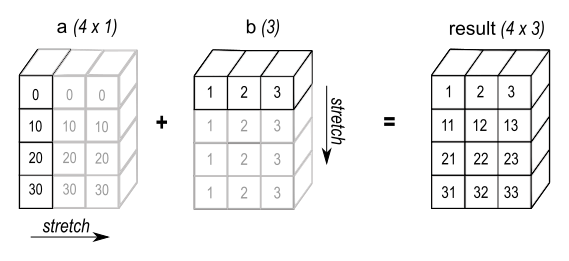
\includegraphics[width=.7\textwidth]{figures/broadcasting_outer.png}
    \caption{Outer sum of two one-dimensional arrays using array broadcasting}
    \label{fig:broadcasting4}
\end{figure}

\end{itemize}

Another way we can think about array broadcasting is that we start at the outermost dimension and work our way in, either multiplying intermediate arrays elementwise or broadcasting a single element to match the size of a multi-dimensional element. 
To see this, let's consider the following two arrays:

\begin{align*}
x = \textcolor{blue}{[} \textcolor{orange}{[} 1 \textcolor{orange}{]}, \\
\textcolor{orange}{[} 2 \textcolor{orange}{]} \textcolor{blue}{]} \\
\end{align*} 

\begin{align*}
 y = \textcolor{blue}{[} \textcolor{orange}{[} 3, 4 \textcolor{orange}{]} \textcolor{blue}{]}
\end{align*}

To multiply these two arrays together using array broadcasting, we start at the outermost dimension of the arrays and then work our way inward.
In this case, the outermost dimension (axis=0) of our arrays is colored in blue, and the inner dimension (axis=1) is colored in orange.

Starting with $x$, there are two objects (the two orange arrays) inside of the blue brackets. 
In $y$, there is only one object in the blue brackets (the one orange array). 
Thus, we will distribute the one orange array in $y$ to the two orange arrays in $x$. For now, we will outline these two arrays with blank arrays as place holders.

\begin{align*}
\textcolor{blue}{[} \textcolor{orange}{[} \textcolor{orange}{]}, \\
\textcolor{orange}{[} \textcolor{orange}{]} \textcolor{blue}{]}\\
\end{align*}

Performing the first multiplication of orange arrays, there is one element in the orange array from $x$ (the number $1$) and two elements in the orange array from $y$ (the numbers $3$ and $4$). 
We will thus distribute the single element from $x$ to the two elements of $y$ by multiplying them elementwise.
The result of this is shown below:

\begin{align*}
\textcolor{blue}{[} \textcolor{orange}{[} 3, 4 \textcolor{orange}{]}, \\
\textcolor{orange}{[} \textcolor{orange}{]} \textcolor{blue}{]}\\
\end{align*}

Performing the second multiplication of orange arrays is similar. The one element of the array from $x$ (the number $2$) is distributed to the two elements from the array in $y$ (the numbers $3$ and $4$) and multiplied by each of them individually. 
The result of this multiplication is shown below:

\begin{align*}
A = \textcolor{blue}{[} \textcolor{orange}{[} 3, 4 \textcolor{orange}{]}, \\
\textcolor{orange}{[} 6, 8 \textcolor{orange}{]} \textcolor{blue}{]}\\
\end{align*}

These are some simple examples of array broadcasting. 
Much more complicated cases come up all the time in scientific computing.
However, by lining up dimensions appropriately, many loops can be turned into elementwise broadcasting operations.
This, in turn, saves a significant amount of time compared to using a for loop to accomplish the same task.


\section*{Numerical Computing with NumPy} % ===================================

\subsection*{Universal Functions} % -------------------------------------------

A \emph{universal function} is one that operates on an entire array element-wise.
Universal functions are significantly more efficient than using a loop to operate individually on each element of an array.

\begin{table}[H]
\centering
\begin{tabular}{r|l}
    Function & Description \\
    \hline
    \li{<<abs()>>} or \li{absolute()} & Calculate the absolute value element-wise. \\
    % \li{conj()} & Return the complex conjugate of the array.\\
    \li{exp()} / \li{log()} & Exponential ($e^x$) / natural log element-wise.\\
    \li{maximum()} / \li{minimum()}& Element-wise maximum / minimum of two arrays.\\
    % \li{<<round()>>} & Return a rounded version of the array.\\
    \li{sqrt()} & The positive square-root, element-wise.\\
    \li{sin()}, \li{cos()}, \li{tan()}, etc. & Element-wise trigonometric operations.
\end{tabular}
\end{table}

\begin{lstlisting}
>>> x = np.arange(-2,3)
>>> print(x, np.<<abs>>(x))             # Like np.array([abs(i) for i in x]).
[-2 -1  0  1  2] [2 1 0 1 2]

>>> np.sin(x)                       # Like np.array([math.sin(i) for i in x]).
array([-0.90929743, -0.84147098,  0.        ,  0.84147098,  0.90929743])
\end{lstlisting}

\begin{problem}
Write a function that accepts a universal function and an $n\times n$ NumPy array, and returns how many times as fast it is to operate on the entire array element-wise, rather than by using a nested for loop to operate on each element individually. 
Run each way of operating on the matrix 10 times, and return the ratio of the averages of the two methods. 
Vow that you will avoid unnecessary nested for loops, especially when operating on large arrays.
\end{problem}

See \url{http://docs.scipy.org/doc/numpy/reference/ufuncs.html#available-ufuncs} for a more comprehensive list of universal functions.

\begin{warn}
The \li{math} module has many useful functions for numerical computations.
However, most of these functions can only act on single numbers, not on arrays.
NumPy functions can act on either scalars or entire arrays, but \li{math} functions tend to be a little faster for acting on scalars.
\begin{lstlisting}
>>> import math

# Math and NumPy functions can both operate on scalars.
>>> print(math.exp(3), np.exp(3))
20.085536923187668 20.0855369232

# However, math functions cannot operate on arrays.
>>> x = np.arange(-2, 3)
>>> np.tan(x)
array([ 2.18503986, -1.55740772,  0.        ,  1.55740772, -2.18503986])
>>> math.tan(x)
<<Traceback (most recent call last):
  File "<stdin>", line 1, in <module>
TypeError: only length-1 arrays can be converted to Python scalars>>
\end{lstlisting}
Always use universal NumPy functions, not the \li{math} module, when working with arrays.
\end{warn}

\subsection*{Other Array Methods} % -------------------------------------------

The \li{np.ndarray} class itself has many useful methods for numerical computations.

\begin{table}[H]
\centering
\begin{tabular}{r|l}
    Method & Returns \\
    \hline
    \li{<<all()>>} & \li{True} if all elements evaluate to \li{True}.\\
    \li{<<any()>>} & \li{True} if any elements evaluate to \li{True}.\\
    \li{argmax()} & Index of the maximum value.\\
    \li{argmin()} & Index of the minimum value.\\
    \li{argsort()} & Indices that would sort the array.\\
    \li{clip()} & restrict values in an array to fit within a given range\\
    \li{<<max()>>} & The maximum element of the array.\\
    \li{mean()} & The average value of the array.\\
    \li{<<min()>>} & The minimum element of the array.\\
    \li{roll()} & shuffles the elements of the array according to specified amount.\\
    \li{sort()} & Return nothing; sort the array in-place.\\
    \li{std()} & The standard deviation of the array.\\
    \li{<<sum()>>} & The sum of the elements of the array.\\
    % \li{trace()} & return the sum of the elements along the main diagonal\\
    \li{var()} & The variance of the array.\\
\end{tabular}
\end{table}

Each of these \li{np.ndarray} methods has an equivalent NumPy function.
For example, \li{A.<<max>>()} and \li{np.<<max>>(A)} operate the same way.
The one exception is the \li{sort()} function: \li{np.sort()} returns a sorted copy of the array, while \li{A.sort()} sorts the array in-place and returns nothing.

Every method listed can operate \emph{along an axis} via the keyword argument \li{axis}.
If \li{axis} is specified for a method on an $n$-D array, the return value is an $(n-1)$-D array, the specified axis having been collapsed in the evaluation process.
If \li{axis} is not specified, the return value is usually a scalar.

\begin{lstlisting}
>>> A = np.arange(9).reshape((3,3))
>>> A
array([[0, 1, 2],
       [3, 4, 5],
       [6, 7, 8]])

# Find the maximum value in the entire array.
>>> A.<<max>>()
8

# Find the minimum value of each column.
>>> A.<<min>>(axis=0)                   # np.array([min(A[:,i]) for i in range(3)])
array([0, 1, 2])

# Compute the sum of each row.
>>> A.<<sum>>(axis=1)                   # np.array([sum(A[i,:]) for i in range(3)])
array([3, 12, 21])
\end{lstlisting}

Similar to the above discussion about array broadcasting, we can color the arrays to gain more visual intuition for how operations can be performed across axes. 

Consider again the array
\begin{align*}
A = \textcolor{blue}{[} \textcolor{orange}{[} 3, 4 \textcolor{orange}{]}, \\
\textcolor{orange}{[} 6, 8 \textcolor{orange}{]} \textcolor{blue}{]}
\end{align*}

Suppose that we wanted to evaluate the call \li{B = np.sum(A, axis = 1)}. 
Axis dimensions are numbered from outmost to inmost so in our case axis 0 denotes the blue brackets and axis 1 denotes the orange brackets.
Summing over axis 1 means that we sum everything in the orange brackets, but leave the result where it lies in the larger array.
So in this case the result would be:
\begin{align*}
B = \textcolor{blue}{[} 7, 14 \textcolor{blue}{]}
\end{align*}

If we instead wanted to compute the sum  \li{B = np.sum(A, axis = 0)}, we would sum the things inside of the blue brackets. 
In this case, there are two things inside of the blue brackets (the two orange arrays). 
These are summed elementwise, resulting in the following array:
\begin{align*}
B = \textcolor{orange}{[} 9, 12 \textcolor{orange}{]}
\end{align*}


Refer to the NumPy Visual Guide in the appendix for more visual examples.

Also see \url{http://docs.scipy.org/doc/numpy/reference/generated/numpy.ndarray.
html} for a more comprehensive list of array methods.


\begin{problem} % Row stochastic matrices.
A matrix is called \emph{row-stochastic}\footnote{Similarly, a matrix is called \emph{column-stochastic} if its columns each sum to $1$.} if its rows each sum to $1$.
Stochastic matrices are fundamentally important for finite discrete random processes and some machine learning algorithms.

Write a function than accepts a matrix (as a 2-D NumPy array).
Divide each row of the matrix by the row sum and return the new row-stochastic matrix.
Use array broadcasting and the \li{axis} argument instead of a loop.
\end{problem}

\subsection*{Vectorizing functions}

Whenever possible making your functions `numpy aware' can greatly reduce complexity, increase readability and simplicity of code and make functions more versatile. 
Designing functions to be able to work with and utilize numpy arrays and numpy functions is one of the best ways to optimize code. 
However, sometimes the functions we need to use are very difficult to vectorize. 
In this case it can be useful to employ \li{np.vectorize()}

\li{np.vectorize()} accepts as an argument a function whose input and output is a scalar. 
It returns a new function that is `numpy aware', meaning that it will accept a numpy array of values and output an array where each entry had the operation defined by the original function performed on it.

\begin{lstlisting}
# Define a function to double a number
>>> def Double(x):           
...		return 2*x

>>> test = np.array([1,2,3,4,5])
# Using a for loop we can get the doubled array
>>> for i,val in enumerate(test):   
...		test[i] *= 2
>>> test
array([2,4,6,8,10])

# Vectorizing our Double function
>>> DoubleVectorized = np.vectorize(Double)   

>>> test = np.array([1,2,3,4,5])
# with the function vectorized the implementation is simple
>>> DoubleVectorized(test)     
array([2,4,6,8,10])

\end{lstlisting}

\begin{info} %warning that this function does not actually help with complexity

While the above example can easily be done with array broadcasting, \li{np.vectorize()} can be implemented with very complex scalar functions for which no array broadcasting method exists. 
However, it should be noted that this function is used only for convenience and readability since it does not improve temporal complexity like normal array broadcasting would. 
Even though it doesn't improve the complexity, it is often simpler than trying to formulate the for loop.

\end{info}


\begin{warn}

Note that \li{np.vectorize()} will infer the type of its output based on the first element of the input.
This behavior can cause confusing results if multiple return types are used within one function.
Make sure to either use the same return type in all branches of the function to be vectorized or specify a return type with the \li{otypes} keyword argument.
The following example illustrates the importance of carefully handling datatypes:


\begin{lstlisting}
def half_heavyside(x):
	if (x > 0):
		return 0.5
	else:
		return 0

>>> f = np.vectorize(half_heavyside)	

>>> f([-1., -0.5, 0., 0.5, 1.])
array([0, 0, 0, 0, 0])

\end{lstlisting}

At first glance, it looks like \li{np.vectorize()} is simply broken. 
However, what is actually happening is \li{np.vectorize()} is infering the datatype from our first input. 
Since the first input, \li{-1}, returned \li{0} (an integer), \li{np.vectorize()} assumes that all subsequent outputs will be of type \li{int} as well. 
When \li{half_heavyside} does return a \li{0.5}, the \li{float} is cast to an \li{int}, thus returning a \li{0}. 

Two example fixes for this problem are shown below. 
The first fix explicitly ensures both return statements are of type \li{float}.
The second fix uses the \li{otypes} keyword argument of \li{np.vectorize()} to specify the correct return type.
Only one type per return value of the wrapped function may be specified with \li{otypes}. 

\begin{lstlisting}
def half_heavyside(x):
	if (x > 0):
		return 0.5
	else:
		return 0.

>>> f = np.vectorize(half_heavyside)	

>>> f([-1., -0.5, 0., 0.5, 1.])
array([0. , 0. , 0. , 0.5, 0.5])

\end{lstlisting}

\begin{lstlisting}
def half_heavyside(x):
	if (x > 0):
		return 0.5
	else:
		return 0

>>> f = np.vectorize(half_heavyside, otypes = [float])	

>>> f([-1., -0.5, 0., 0.5, 1.])
array([0. , 0. , 0. , 0.5, 0.5])

\end{lstlisting}

\end{warn}

\begin{problem}

Given to you is the code that finds the prime factorization of a number and returns the largest prime in the factorization. 
Vectorize the function using \li{np.vectorize()} and program a function that either uses the vectorized function or the naive for loop depending on the argument `naive' being passed in as True or False. 

Make sure you function returns a numpy array of the same size for both cases.

\noindent Hint: Make sure the naive approach returns the array with a dtype of `int32'

\end{problem}

\section*{Einsum}

While numpy has many functions to help multiply arrays, multiplying the elements of arrays in unorthodox ways usually requires the conglomeration of quite a few of these functions. 
\li{np.einsum()} is designed to eliminate this problem by making a general framework for multiplication and addition in arrays using their shapes and allowing the coder to tell the function which elements exactly are to be multiplied or summed and how those operations are to be returned.

\subsection*{Einsteinian summation notation}
The function name \li{einsum()} comes from the term \emph{Einsteinian summation}, which is a standard notational technique in physics and engineering for matrix and tensor operations.

To understand how this works, consider the simple operation of the dot product $\mathbf{x} \cdot \mathbf{y}$, where $\mathbf{x}, \mathbf{y} \in \mathbb{R}^n$.
As we know, this is defined as 

\begin{align*}
\mathbf{x} \boldsymbol{\cdot} \mathbf{y} = \sum_{i=1}^{n} x_i y_i
\end{align*}

In the equation above, the $i$ is what we refer to as a \emph{dummy index}; that is, $i$ is only used inside the sum, and never appears outside the sum. 

As another example, consider the operation of matrix multiplication. 
Given $A \in M_{n \times m}(\mathbb{R})$ and $B \in M_{m \times \ell} (\mathbb{R})$, we know that the $ij$-element of the resulting matrix product $AB \in M_{n \times \ell}(\mathbb{R})$ is given by
\begin{align*}
[AB]_{ij} = \sum_{k=1}^{m} a_{ik}b_{kj}
\end{align*}

Again, since $k$ only appears inside the summation, it is a dummy index. 
However, $i$ and $j$ appear on both the left and right hand sides of this equation, so they are called \emph{free indexes} (and they are not summed over).

Notice that, in both of these examples, we have written vector-valued and matrix-valued operations, respectively, by denoting what an element of the output array should look like in terms of indexes.
In the dot product example, the output is a scalar, so we have denoted what the scalar should be in terms of the elements of the input vectors to that operation.
In the matrix multiplication example, the output is a matrix, so we have denoted what each $ij$ element of that matrix should be in terms of the elements of the input matrices to that operation.

In essence, Einsteinian summation notation does exactly this: it denotes what a given element of the output array should be in terms of the elements of the input array, just as we have done above.
However, for brevity, all summation symbols are dropped in this notation, and all dummy indexes are implicitly summed over.

In this notation, the dot product would be written
\begin{align*}
\mathbf{x} \boldsymbol{\cdot} \mathbf{y} = x_i y_i
\end{align*}

Similarly, the matrix product would be written
\begin{align*}
[AB]_{ij} = a_{ik}b_{kj}
\end{align*}

For this reason, Einsteinian summation notation is often called \emph{index notation}.

Notice that clever, unorthodox ways of taking ``products'' of matrices and vectors can be defined in this way.
For example, given two matrices  $A \in M_{n \times m}(\mathbb{R})$ and $B \in M_{m \times n} (\mathbb{R})$, we can define a clever product $A \odot B$ that (1) takes the normal matrix product and (2) takes the trace of that resulting matrix as
\begin{align*}
A \odot B = \sum_{i=1}^{n}[AB]_{ii} = \sum_{i=1}^{n} \sum_{k=1}^{m} a_{ik} b_{ki}
\end{align*}
By noting that $i$ and $k$ are now dummy variables, and the output is a scalar, we can write this unusual product in index notation as
\begin{align*}
A \odot B = a_{ik} b_{ki}
\end{align*}


\begin{info}
In traditional index notation, the only time an index is summed over is when it appears twice in an expression, such as the index $i$ in the dot product $\mathbf{u} \boldsymbol{\cdot} \mathbf{v} = u_i v_i$. Thus, the only things considered ``dummy indexes'' are indexes which appear twice in an expression.

\noindent However, there are many more expressions that we can represent by summing over indexes which are not repeated. 
For example, we can take a row sum of a $m \times n$ matrix $A$, resulting in the $m$-dimensional vector $\mathbf{v}$, using the following rule:
\begin{align*}
	[v]_i &= \sum_{j=1}^{n} a_{ij}
\end{align*}
Note that we are summing over $j$ here, but it is not a repeated index. 
So this expression would not be representable in traditional index notation without a much more convoluted expression.

\noindent Despite this limitataion, such an expression \emph{is} representable using \li{np.einsum()}, as we will describe in the next section.
So, while the notation of  \li{np.einsum()} is similar to that of traditional index notation, it is more flexible. 

\noindent So, through the rest of this manual, we will write mathematical development of these expressions with summation notation, rather than index notation, to make clear exactly what variables are being summed over (that is, to distinguish between free variables and dummy variables).

\end{info}


\subsection*{Numpy's Einsum}

The function \li{np.einsum()} is a function which is designed to be used with operations defined in terms of Einsteinian summation notation, defined in the previous section.
It can be used on arrays of higher dimensions, but we'll keep the scope of this section to working with input arrays of 1 or 2 dimensions. 

The numbers in the following syntax only represent positions, each position will be explained below:

\begin{center}
\li{np.einsum("12,34 -> 56", 7, 8)}
\end{center}

The meaning of the positions are as follows:

\begin{enumerate}
\item[\textcolor{magenta}{1} and \textcolor{magenta}{2})] Symbols representing the index of an element in the first input array. In the case of 1 dimensional vectors, there will only be one variable and the second will be omitted.
\item[\textcolor{magenta}{3} and \textcolor{magenta}{4})] Similarly, symbols representing the index of an element in the second input array.
\item[\textcolor{magenta}{5} and \textcolor{magenta}{6})] Symbols representing the index of an item in the output array. There can zero (for scalars), one (for vectors), two (for matrices), or even three (for higher-order tensors) variables here.
\item[\textcolor{white}{easter} \textcolor{magenta}{7})] The first input array. Make sure it is outside the quotation mark ending the variables section and preceded by a comma.
\item[\textcolor{white}{e g g!} \textcolor{magenta}{8})] The second input array.
\end{enumerate}

Positions 7 and 8 are obviously arrays, but position 1-6 are filled with textual symbols, usually $i$, $j$, and $k$, which represent the indexes of elements in the input and output arrays. 

\textbf{The key here} is that we can translate anything in summation notation to an einsum expression.
To do this, the subscripts of anything \emph{inside} the summation are the letters on the left-hand side of the arrow, with commas separating different quantities. 
The subscripts of anything on the \emph{result} of a summation notation expression are the letters on the right-hand side of the arrow.
This idea will be demonstrated more fully in the following section.

\subsection*{Einsum Rules}

The way \li{einsum()} interprets its inputted variables are as follows:

\begin{enumerate}
\item[1)] If the variables contained in positions 1 or 2 share a variable in 3 or 4, the values along the axes specified by the repeated variables positions will be multiplied together\\
\item[2)] On the other side of the arrow (positions 5 and 6), specify the dimensions of the output. 
Ommiting a variable from these positions causes the products to be summed. 

(That is, any variables that appear on both sides of the arrow are free variables, and any variables only on the left-hand side are dummy variables that are summed over).
\end{enumerate}
\noindent As an example, we will define normal matrix multiplication using einsum. 
Recall that the summation notation for this (rewritten with a different dummy index) is 
\begin{align*}
[AB]_{ik} = \sum_{j=1}^{m }a_{ij}b_{jk}
\end{align*}

This means that the following \li{np.einsum()} command will perform normal matrix multiplication:
\begin{lstlisting}
>>> import numpy as np

>>> A = np.eye(3)
>>> A[0,:] += A[2,:]
>>> A
array([[1, 0, 1],
       [0, 1, 0],
       [0, 0, 1]])

>>> B = np.arange(9).reshape((3,3))
>>> B
array([[0, 1, 2],
       [3, 4, 5],
       [6, 7, 8]])

# We use einsum to define normal matrix multiplication
# note the 'j' is repeated in axis 1 and axis 0 respectively
>>> np.einsum("ij,jk -> ik", A, B) 
array([[6, 8, 10],
       [3, 4, 5],
       [6, 7, 8]])

\end{lstlisting}

Since the \li{j} was repeated in the previous example, the elements on those 2 axes are paired and multiplied together elementwise.
The first pair of indicies has \li{j} in the second position, which corresponds to the column position (axis=1; moving from column to column down a single row). 
The second pair of indices has \li{j} in the first position, which corresponds to the row position (axis=0; moving row to row down a single column). 
Thus, Einsum takes the elementwise products of the elements along each respective row of \li{A} and column of \li{B}. This corresponds to the $a_{ij}b_{jk}$ in the summation notation, above.

Additionally, the output indexes were specified to be \li{ik} instead of \li{ijk}. 
Therefore, since $j$ was present on the left-hand-side of the Einsum expression, and not the right-hand side, the elementwise products $a_{ij}b_{jk}$  were summed over all of the $j$ indexes (exactly as defined in the summation notation above). 

It's important to note here that Einsum adds and multiplies in a very similar manner to the \li{axis} argument in \li{np.sum()} and other numpy functions.

\subsection*{Common operations using Einsum}

The below table describes some classical operations on vectors and matrices, and how they may be defined in terms of (1) summation notation and (2) the corresponding \li{np.einsum()} command.

\begin{table}[H]
\centering
\begin{tabular}{|m{0.35\linewidth} | m{0.25\linewidth} | m{0.4\linewidth}|}
    \hline
    \text{Operation} & Summation Notation & Einsum Command \\
    \hline
    \hline
    Transpose of a matrix $A$ & $[A^\intercal]_{ij} = a_{ji}$ & \li{np.einsum("ji -> ij", A)} \\
    \hline
    Row sum vector $r$ of a matrix $A$ & $[r]_{i} = \sum_{j=1}^{m} a_{ij}$ & \li{np.einsum("ij -> i", A)} \\
    \hline
    Column sum vector $c$ of a matrix $A$ & $[c]_{j} = \sum_{i=1}^{n} a_{ij} $ & \li{np.einsum("ij -> j", A)} \\
    \hline
    Sum $s$ of all elements of a matrix $A$ & $s = \sum_{i=1}^{n} \sum_{j=1}^{m} a_{ij}$ & \li{np.einsum("ij->",A)} \\
    \hline
    Trace of a matrix $A$ & $\operatorname{tr}(A) = \sum_{i=1}^{n} a_{ii}$ & \li{np.einsum("ii->", A)}\\
    \hline
    Dot product of $u$ and $v$ & $u \boldsymbol{\cdot} v = \sum_{i=1}^{n} u_i v_i$ & \li{np.einsum("i, i ->", x, y)} \\ 
    \hline
    Outer product of $u$ and $v$ & $[u \otimes v]_{ij} = u_{i}v_{j}$ & \li{np.einsum("i, j -> ij", u, v)} \\
    \hline
    Matrix product of $A$ and $B$ & $[AB]_{ik} = \sum_{j=1}^{n} a_{ij}b_{jk} $ & \li{np.einsum("ij, jk -> ik", A, B)} \\
    \hline
    Elementwise product $B$ of a vector $u$ by each \emph{row} of a matrix $A$ & $[B]_{ij} = a_{ij}u_{j}$ & \li{np.einsum("ij, j -> ij", A, u)} \\
    \hline
    Elementwise product $B$ of a vector $v$ by each \emph{column} of a matrix $A$ & $[B]_{ij} = a_{ij}v_{i}$ & \li{np.einsum("ij, i -> ij", A, v)} \\
    \hline
\end{tabular}
\end{table}


\begin{info}
Notice again that excluding a letter after the \li{->} symbol will cause summation of the specified scalar products along the axis whose letter was excluded.
On the other hand, including a letter after the \li{->} symbol will \emph{disallow} summation along that index, and will instead create an output dimension of the same size as the input dimension corresponding to that letter.

\noindent For example, see the row sum entry in the above table.
Since the row index \li{i} is included after the \li{->} symbol, the resulting vector will have the same dimension as the number of rows.
However, since the column index \li{j} is \emph{not} included after the \li{->} symbol, the scalar values $a_{ij}$ must be summed over all \li{j} values corrresponding to each \li{i} value before they are output. 
This corresponds to summing over all of the columns in the \li{i}th row before storing the output in the \li{i}th entry of the output vector.
\end{info}

\subsection*{A longer example}

Now, to demonstrate Einsum's true power we'll show a more complicated example. 

Imagine you needed to take an outer product of each column of a matrix $A \in M_{n,m}(\mathbb{R})$ with the corresponding column of another matrix $B \in M_{\ell,m}(\mathbb{R})$, storing the result in an array called \li{outer_products}, where \li{outer_products[k]} is defined to be the $n \times \ell$ outer product array of the $k$th column of $A$ with the $k$th column of $B$ for every $1 \leq k \leq m$.

You could accomplish this in a for loop, but it would be slow and not very effective. 
Conversely, this can be done in one line with \li{np.einsum}, with the correct mathematical setup.

Let $\mathbf{u}_k$ being the $k$th column of $A$, and $ \mathbf{v}_k$ be the corresponding $k$th column of $B$. 
We look to find the outer product
\begin{align*}
	[\mathbf{u}_k \otimes \mathbf{v}_k]_{ij} = [u_{k}]_{i} [v_{k}]_{j}, \quad 1 \leq i \leq n, 1 \leq j \leq \ell
\end{align*}
for $1 \leq k \leq m$.

We know that the $i$th element of $\mathbf{u}_k$ (the $k$th column of $A$) is just $a_{ik}$. Similarly, the $j$th element of $\mathbf{v}_{k}$ (the $k$th column of $B$) is just $b_{jk}$. Substituting these values into the above expression

\begin{align*}
	[\mathbf{u}_k \otimes \mathbf{v}_k]_{ij} = a_{ik} b_{jk}, \quad 1 \leq i \leq n, 1 \leq j \leq \ell
\end{align*}

Finally, letting $C$ denote the three-dimensional array \li{outer_products}, we have found that 
\begin{align*}
	[C]_{kij} = [\mathbf{u}_k \otimes \mathbf{v}_k]_{ij} =  a_{ik} b_{jk}
\end{align*}

This is already in index notation, which allows us to write the corresponding Einsum expression in one line:

\begin{lstlisting}
>>> A = np.arange(9).reshape((3,3))
>>> B = np.arange(12).reshape((4,3))
# Notice these are just the indexes from the final index notation expression
>>> outer_products = np.einsum("ik, jk -> kij", A, B)
>>> outer_products
array([[[ 0,  0,  0,  0],
        [ 0,  9, 18, 27],
        [ 0, 18, 36, 54]],

       [[ 1,  4,  7, 10],
        [ 4, 16, 28, 40],
        [ 7, 28, 49, 70]],

       [[ 4, 10, 16, 22],
        [10, 25, 40, 55],
        [16, 40, 64, 88]]])
\end{lstlisting} 

The output dimension having three variables creates a 3-dimensional matrix where each element in the first axis is a 3 by 4 outer product matrix. 

If we then wanted to sum the rows of each of those outer-product matrices, resulting in a $k \times n$ array of row sums, notice that we would want an output array $C$ such that 
\begin{align*}
	[C]_{ki} = \sum_{j=1}^{n} [\mathbf{u}_k \otimes \mathbf{v}_k]_{ij} =  \sum_{j=1}^{n} a_{ik} b_{jk}
\end{align*}
Notice now that $j$ has become a dummy variable, and thus, we must eliminate it from the right-hand side of the arrow in the Einsum expression:
\begin{lstlisting}
>>> A = np.arange(9).reshape((3,3))
>>> B = np.arange(12).reshape((4,3))
>>> outer_products_sum = np.einsum("ik, jk -> ki", A, B)
>>> outer_products_sum
array([[  0,  54, 108],
       [ 22,  88, 154],
       [ 52, 130, 208]])
\end{lstlisting}

Finally, perhaps we want to multiply a different vector $\mathbf{v}$ elementwise to the rows of this resulting \li{outer_products_sum} array. 
That is (again letting $[C]_{ki}$ denote the output elements of this output array), we want the $i$th element of $v$ to be multiplied by our earlier expression for $[C]_{ki}$:
\begin{align*}
[C]_{ki} = \left(\sum_{j=1}^{n} a_{ik} b_{jk} \right)v_i = \sum_{j=1}^{n} a_{ik} b_{jk} v_i
\end{align*} 

The resulting code displays the results:
\begin{lstlisting}
>>> A = np.arange(9).reshape((3,3))
>>> B = np.arange(12).reshape((4,3))
>>> v = np.array([0,1,-1])
>>> outer_products_with_broadcast = np.einsum("ik, jk, i -> ki", A, B, v)
>>> outer_products_with_broadcast
array([[   0,   54, -108],
       [   0,   88, -154],
       [   0,  130, -208]])
\end{lstlisting}

\noindent Thus, three difficult operations have been reduced to a few letters by the power of \li{np.einsum()}.

\subsection*{Einsum Optimize}

\li{np.einsum()}, in most cases, performs faster than built in numpy functions. 
However, the way Einsum organizes its operations creates redundancy when trying to perfrom multiple operations at once, such as multiplying two matrices, broadcasting a vector to its rows and then summing the resulting matrix columns. 
One should be cautious when using Einsum to perform multiple operations since you may actually be making your complexity worse rather than improving it. 

There are two ways around this problem. 
First, performing each operation individually will preserve the integrity of Einsum's performance, although brevity of code will suffer. 
Second, multiple operations can be performed efficiently using kwarg \li{optimize=True}.

Setting \li{optimize=True} creates an extra step of operational analysis before any calculations are made to ensure efficient order of operations. 
In addition, this mode uses a more spatially complex method of computation in exchange for ensured temporal gains. 
This is why \li{optimize} defaults to \li{False}: to allow the programmer to know whether or not there is sufficient memory or need for the optimize functionality.

\begin{problem}
Write a function that accepts 3 vectors and a matrix of appropriate sizes and returns a matrix that is the result of an outer product of the first 2 vectors, the 3rd vector array broadcast multiplied onto the columns of that matrix and then the multiplication via normal matrix multiplication of that result to the inputed matrix. 
Your function should take a keyword argument \li{split} that defaults to \li{False}. If \li{split=True}, then the einsum operations should be performed one at a time. 
Otherwise, the operations should be performed all at once while using \li{optimize=True}.

Write an additional function that performs the same operations only using numpy operations. 

Hint: Your result should return the equivalent of \li{np.outer(x,y)*z.reshape(-1,1)@A} where \li{x}, \li{y}, and \li{z} are vectors and \li{A} is a matrix.
\label{prob:outer product}
\end{problem}

\begin{problem}
Time your einsum function from Problem \ref{prob:outer product} versus its numpy function equivalent for vectors of size 3 through 500 and arrays of size (3,3) through (500,500). 
You should time your einsum function both with and without \li{split=True}. 
Plot the results on a neatly formatted and labeled graph. 
Compare your results to Figure \ref{fig:einsum}.
\begin{figure}[H]
    \includegraphics[width=.7\textwidth]{figures/einsum_timing.pdf}
    \caption{}
    \label{fig:einsum}
\end{figure}
\end{problem}

\newpage

\section*{Additional Material} % ==============================================

\subsection*{Random Sampling} % -----------------------------------------------

The submodule \li{np.random} holds many functions for creating arrays of random values chosen from probability distributions such as the uniform, normal, and multinomial distributions.
It also contains some utility functions for getting non-distributional random samples, such as random integers or random samples from a given array.

\begin{table}[H] % The np.random submodule.
\begin{tabular}{r|l}
Function & Description\\
\hline
\li{choice()} & Take random samples from a 1-D array.\\
\li{random()} & Uniformly distributed floats over [0, 1).\\
\li{randint()} & Random integers over a half-open interval.\\
\li{random_integers()} & Random integers over a closed interval.\\
\li{randn()} & Sample from the standard normal distribution.\\
\li{permutation()} & Randomly permute a sequence / generate a random sequence.\\
\\
Function & Distribution\\
\hline
\li{beta()} & Beta distribution over [0, 1].\\
\li{binomial()} & Binomial distribution.\\
\li{exponential()} & Exponential distribution.\\
\li{gamma()} & Gamma distribution.\\
\li{geometric()} & Geometric distribution.\\
\li{multinomial()} & Multivariate generalization of the binomial distribution.\\
\li{multivariate_normal()} & Multivariate generalization of the normal distribution.\\
\li{normal()} & Normal / Gaussian distribution.\\
\li{poisson()} & Poisson distribution.\\
\li{uniform()} & Uniform distribution.
\end{tabular}
\end{table}

Note that many of these functions have counterparts in the standard library's \li{random} module.
These NumPy functions, however, are much better suited for working with large collections of random samples.

\begin{lstlisting}
# 5 uniformly distributed values in the interval [0, 1).
>>> np.random.random(5)
array([ 0.21845499,  0.73352537,  0.28064456,  0.66878454,  0.44138609])

# A 2x5 matrix (2-D array) of integers in the interval [10, 20).
>>> np.random.randint(10, 20, (2,5))
array([[17, 12, 13, 13, 18],
       [16, 10, 12, 18, 12]])
\end{lstlisting}


\subsection*{Saving and Loading Arrays} % -------------------------------------

It is often useful to save an array as a file for later use.
NumPy provides several easy methods for saving and loading array data.

\begin{table}[H]
\begin{tabular}{r|l}
Function & Description\\
\hline
\li{save()} & Save a single array to a \texttt{.npy} file.\\
\li{savez()} & Save multiple arrays to a \texttt{.npz} file.\\
\li{savetxt()} & Save a single array to a \texttt{.txt} file.\\
\hline
\li{load()} & Load and return an array or arrays from a \texttt{.npy} or \texttt{.npz} file.\\
\li{loadtxt()} & Load and return an array from a text file.
\end{tabular}
\end{table}

\begin{lstlisting}
# Save a 100x100 matrix of uniformly distributed random values.
>>> x = np.random.random((100,100))
>>> np.save("uniform.npy", x)       # Or np.savetxt("uniform.txt", x).

# Read the array from the file and check that it matches the original.
>>> y = np.load("uniform.npy")      # Or np.loadtxt("uniform.txt").
>>> np.allclose(x, y)               # Check that x and y are close entry-wise.
<<True>>
\end{lstlisting}

To save several arrays to a single file, specify a keyword argument for each array in \li{np.savez()}.
Then \li{np.load()} will return a dictionary-like object with the keyword parameter names from the save command as the keys.

\begin{lstlisting}
# Save two 100x100 matrices of normally distributed random values.
>>> x = np.random.randn(100,100)
>>> y = np.random.randn(100,100)
>>> np.savez("normal.npz", first=x, second=y)

# Read the arrays from the file and check that they match the original.
>>> arrays = np.load("normal.npz")
>>> np.allclose(x, arrays["first"])
<<True>>
>>> np.allclose(y, arrays["second"])
<<True>>
\end{lstlisting}


\subsection*{Polynomials} % ---------------------------------------------------

The \li{np.poly1d} object represents a polynomial in NumPy.
The constructor is called with the coefficients of the desired polynomial.

\begin{lstlisting}
>>> poly = np.poly1d([3, 5, 1, 2, 0, 1])
>>> print(poly)
   5     4     3     2
3 x + 5 x + 1 x + 2 x + 1
\end{lstlisting}

The object \li{poly} represents the polynomial $3x^5+5x^4+x^3+2x^2+1$.
NumPy provides many functions to operate on \li{poly1d} objects (see \url{http://docs.scipy.org/doc/numpy/reference/routines.polynomials.polynomial.html}).

Recall that
\[
e^x = \sum_{n=0}^{\infty} \frac{x^n}{n!}.
\]
The following function evaluates the $N$th partial sum of this series at the value $a$.

\begin{lstlisting}
>>> from scipy.special import factorial
>>> def exp(a, N=25):
...     """Construct an array in reverse order from n to 0."""
...     n = np.arange(N, -1, -1)
...     # Use broadcasting to compute coefficients
...     coeffs = 1. / factorial(n)
...     poly = np.poly1d(coeffs)        # Make a polynomial object.
...     return poly(a)
...
\end{lstlisting}

The last two lines can be condensed by using the following command:

\begin{lstlisting}
np.polyval(p, a)
\end{lstlisting}

%\begin{problem}
%\leavevmode
%\begin{enumerate}
%\item Use NumPy's polynomial objects to approximate the following series.
%\[
%\arcsin x = \sum_{n=0}^{\infty} \frac{\left(2 n\right) ! x^{2 n + 1}}{\left(2 n + 1\right)\left(n!\right)^2 4^n}
%\]
%This series converges on $(-1, 1)$. Use your series approximation to approximate $\pi$. Hint: think of the powers of $x$ that
%are not included in the series as having zero coefficients.
%
%\item The lambert W function is the inverse of $x e^x$.
%Its Taylor series is below (note the index starts at 1).
%\[
%W(x) = \sum_{n=1}^{\infty} \frac{\left(-n\right)^{n-1} x^n}{n!}
%\]
%This series has a radius of convergence of $\frac{1}{e}$.
%Use the series to approximate a number $x$ such that $x e^x = \frac{1}{4}$.
%Verify that your approximation is close.
%\end{enumerate}
%\end{problem}


\subsection*{Iterating Through Arrays} % --------------------------------------

Iterating through an array (using a \li{for} loop) negates most of the advantages of using NumPy.
Avoid iterating through arrays as much as possible by using array broadcasting and universal functions.
When absolutely necessary, use \li{np.nditer()} to create an efficient iterator for the array.
See \url{http://docs.scipy.org/doc/numpy/reference/arrays.nditer.html} for details.


\subsection*{Expressing Einsum Expressions in Terms of Other Functions} % -------------------------

Conceptually, we can think of \li{np.einsum()} as projecting tensors into higher dimensional space, elementwise multiplying the matrices together, and then summing along the specified dimensions. 
We can thus write many \li{np.einsum()} expressions as a combination of transposes, elementwise multiplications, sums, and expanding dimensions. 
Note that writing \li{np.einsum()} expressions in this way is much less efficient and convenient than just using a call to \li{np.einsum()}. 
This is rather used as an alternate way of understanding what \li{np.einsum()} is doing.
We will work through an example of how this is done to illustrate the concepts.

Consider the following \li{np.einsum()} expression.

\begin{lstlisting}
np.einsum("ijk, jil -> kil", A, B)
\end{lstlisting}

Each of the different letters in the Einsum expression will label a different axis. Since there are four letters, we project into four dimensions.
It doesn't necessarily matter how this axis-to-letter pairing is done, as long as we are consistent, but its often convenient to do it alphabetically. 
We will let \li{i} denote axis 0, \li{j} denote axis 1, \li{k} denote axis 2, and \li{l} denote axis 3. 

We can increase the dimensions of the matrices with a call to \li{np.expand_dims()}. In this case we would call, 

\begin{lstlisting}
A = np.expand_dims(A, 4)

B = np.expand_dims(B, 4)
\end{lstlisting}

We now need to align all the axes of all matrices we are working with.
In our example, with our choice of axis-to-letter pairing, the axes of matrix $A$ are already in the correct alignment. 
We can order the dimensions of B with the following call to \li{np.transpose()}, where the axes passed to \li{np.transpose} correspond to the axis-to-letter pairing that we denoted earlier:

\begin{lstlisting}
B = np.transpose(B, (1,0,3,2))
\end{lstlisting}

After correctly ordering the dimensions, we elementwise multiply the matrices together. 

\begin{lstlisting}
C = A * B
\end{lstlisting}

With our final matrix, we sum along all dimensions that are missing from the output specifier. In our case, since \li{j} is missing, we sum along axis 1. 

\begin{lstlisting}
C = np.sum(C, axis = 1)
\end{lstlisting}

Finally, we  transpose the result so that the axis labels are consistent with the output specifier. Note that \li{k} has now become axis 1 and \li{l} has become axis 2.

\begin{lstlisting}
C = np.transpose(C, (1, 0, 2))
\end{lstlisting}


\subsection*{An Advanced Example of Broadcasting and Einsum} % -------------------------------------
The techniques of array broadcasting and \li{np.einsum()}, while quite daunting at first, constitute an arsenal of extremely powerful techniques that allow you to design algorithms that run quickly on large quantities of data.

Consider the following real-world example, built off of the machine-learning idea of Gaussian Mixture Models (GMMs), which demonstrates the power of using these techniques in tandem.

Assume you have have $n$ data points $\{z_0, \ldots, z_{n-1}\}$, where each data point is $d$-dimensional (that is, $z_i \in \mathbb{R}^d$ for $i = 0, \ldots, n-1$). 

Underlying the phenomenon we are studying, assume there are $K$ multivariate normal distributions $\left\{\mathcal{N}(\mu_0, \Sigma_0), \ldots, \mathcal{N}(\mu_{K-1}, \Sigma_{K-1})\right\}$, each of which contribute with some corresponding weight $\{w_0, \ldots, w_{K-1}\}$ to the full probability distribution:
$$P(z|\theta) = \sum_{k=0}^{K-1} w_k \mathcal{N}(z | \mu_k, \Sigma_k) $$
(where $\mathcal{N}(z | \mu_k, \Sigma_k) $ denotes the standard p.d.f. for the normal distribution with mean $\mu_k$  and covariance $ \Sigma_k $). 

Our goal, given the data points $z_i$, is to figure out which parameters $w_k, \mu_k,$ and $\Sigma_k$ (for $k = 0, \ldots, K-1$) best fit the data. 

Skipping some details, the GMM algorithm iteratively updates guesses for these $3K$ parameters at each timestep $t$.
Specifically, given (1) an updated mean $\mu_k^{t+1}$ and (2) some probabilities $q_i^t(k)$ dependent on (a) the data point $z_i$, (b) the distribution index $k \in [0, \ldots, K-1]$,  and (c) the timestep $t$, the update step for the covariance matrices is given by:
\begin{align*}
	\Sigma_k^{t+1} = \frac{\sum_{i=1}^{n} q_i^t(k) (z_i - \mu_k^{t+1}) (z_i - \mu_k^{t+1})^\top}{\sum_{i=1}^{n} q_i^t(k)}
\end{align*}

The goal of this section will be to describe how to implement this in Python code.

Assume that you have the following arrays available to you, each having to do with one of the three symbols in the right-hand side of the above expression:
\begin{itemize}
	\item \li{q_values} : \li{(K,n)} array with the elements being \li{q_values[k,i]} $ = q_i^t(k)$.
	
	\item \li{Z}: \li{(n,d)} array with each row being \li{Z[i,:]} $ = z_{i} $ 
		
	\item \li{new_means}: \li{(K,d)} array with each row being \li{new_means[k,:]} $= \mu_{k}^{t+1}$
\end{itemize}

We want to store the resulting covariance matrices in an array \li{new_covars}, which will satisfy \li{new_covars[k,:,:]} $= \Sigma_{k}^{t+1}$. Noting that each covariance matrix will be $d \times d$, we can see that \li{new_covars} will have shape \li{(K, d, d)}.

One naive way to implement this would be to use a nested for loop:
\begin{lstlisting}
>>> K, d = new_means.shape
>>> _, n = q_values.shape
>>> new_covars = np.zeros((K,d,d))
>>> for k in range(K):
... 	for i in range(n):
...	        centered = Z[i,:] - new_means[k,:]
...	        outer_prod = np.outer(centered, centered)
...	        new_covars[k,:,:] += q_values[k,i] * outer_prod
...	    new_covars[k,:,:] /= np.sum(q_values[k,:])
\end{lstlisting}

However, this is extremely inefficient, and can take hours to run as the number of data points becomes large.
As a result, this operation calls for some more advanced techniques.

Our goal will be to do this entire operation in a series of array broadcasting steps, using only a single Einsum command.
This will make the code much more efficient.

To do so, we will start by taking bite-size chunks of the expression, figuring out how to write them in code using broadcasting and Einsum.
Then, through a series of steps, we will gradually come up with a formula that will perform the calculation for this expression without a need for any looping whatsoever.

\begin{itemize}
\item \textbf{Step 1:} (Computing the differences between the means $\mu_i$ and the data points $z_k$)

Notice that the numerator contains the expression 
\begin{align*}
(z_i - \mu_k^{t+1})
\end{align*}
more than once.
	
As a first step, we look to create an array called \li{obs_centered} with shape \li{(K,n,d)}, such that \newline \noindent \li{obs_centered[k,i,:]} $ = z_i - \mu_k^{t+1}$. 
	
That is, we want a 3-dimensional array, where each inner element is a 2-dimensional matrix. 
Each 2-dimensional matrix will be produced by subtracting one row of the \li{new_means} matrix from all $n$ rows of \li{Z}.
	
Recall: if we have two 1-dimensional arrays \li{a} and \li{b}, and we want to take the ``outer difference'' between them (that is, we want to create a 2-dimensional array containing the differences of every element of \li{a} with every element of \li{b}), we can do something akin to what is shown in Figure \ref{fig:broadcasting4} and its preceding example:

\begin{lstlisting}
>>> a = np.array([1,2,3])
>>> b = np.array([4,5])
>>> a - b[:,np.newaxis]
array([[-3, -2, -1],
       [-4, -3, -2]])
\end{lstlisting}

Notice that the shapes of the arrays in this broadcast are \li{(3,)} and \li{(2,)}, respectively, and the output shape is \li{(2,3)}.
	
Digging deeper into what's going on here, the broadcasting operation of subtraction (and padding of dimensions) executed the following rearranging of shapes before performing the elementwise subtraction:
	
\begin{lstlisting}
a	:  (3,) -> (1,3) -> (2,3)
b	:  (2,) -> (2,1) -> (2,3)
\end{lstlisting}
	
Now, what we seek to do in our current problem is to take a very similar ``outer difference'' of the \emph{rows} of \li{Z} and \li{new_means}.
This is almost identical to the above case, but instead of subtracting 0-dimensional scalars, we are looking to take the difference between 1-dimensional vectors, each with $d$ elements.
	
Therefore, we look to outer-subtract the $n$ rows of \li{Z} with the $K$ rows of \li{new_means} in all possible combinations, in the exact way we looked to outer-subtract the scalars of the input arrays \li{a} and \li{b} in our example above.

The ultimate output we desire is a \li{(K,n,d)} array (similar to how we ended up with a \li{(2,3)} array in the scalar example).
	
The code in this case is, therefore, nearly identical to the scalar case.
All we need to figure out is how to pad the dimensions of these array in the correct way to get this outer difference of vectors.
This is a bit trickier since having a $d$ in the rightmost slot means we can't just use \li{np.newaxis} as easily as before.
	
Despite this setback, however, looking to the two leftmost dimensions, and leaving the rightmost dimension (the vectors we wish to subtract) alone, comparison to the scalar example shows that we want to achieve the following shapes:
\begin{lstlisting}
Z			: (n,d) -> (1,n,d)
new_means	: (K,d) -> (K,1,d)
\end{lstlisting}
So, what commands to we need to use to achieve these paddings?

The command to add a singleton dimension in the middle of the original shape of \li{new_means} is \li{np.expand_dims(new_means, 1)}.
	
Once that is done, the padding to the left of \li{Z} is automatic by the rules of array broadcasting.

So the desired command is:
\begin{lstlisting}
>>> obs_centered = Z - np.expand_dims(new_means, 1)
\end{lstlisting}


\item \textbf{Step 2:} (Computing the outer products of these differences with themselves)

Notice that there is a term in the numerator of our desired expression that looks like:
\begin{align*}
(z_i - \mu_k^{t+1})(z_i - \mu_k^{t+1})^\top
\end{align*}
This is exactly an outer product of one of the vectors found in Step (1) with itself.

Our goal in this step is to produce an intermediate array \li{outer_products} of shape with shape \li{(K, n, d, d)} such that \li{outer_products[k,i,:,:] } $ = (z_i - \mu_k^{t+1})(z_i - \mu_k^{t+1})^\top$.

Given that \li{obs_centered[k,i,:]} $= (z_i - \mu_k^{t+1})$ by our design, we therefore see that \newline 
\li{outer_products[k,i,:,:]} is just the outer product of \li{obs_centered[k,i,:]} with itself.

In other words,  \newline \li{outer_products[k,i,:, :]} $=$  \li{obs_centered[k,i,:]} $\otimes$ \li{obs_centered[k,i,:]}.

It follows that the $pq$-element of  \li{outer_products[k,i,:, :]} is equal to the $pq$-element of \li{obs_centered[k,i,:]} $\otimes$ \li{obs_centered[k,i,:]}.

Writing this in summation/index notation, letting $u$ denote \li{obs_centered} and $v$ denote \newline \li{outer_products}, we have shown that 
\begin{align*}
v_{kipq} = [v_{ki::}]_{pq} = [u_{ki:} \otimes u_{ki:}]_{pq} = u_{kip} u_{kiq}
\end{align*}
Therefore, we can write the full einsum expression (with all indexes \emph{inside} the expression) as
\begin{lstlisting}
>>> outer_products = np.einsum("kip, kiq -> kipq", obs_centered, obs_centered)
\end{lstlisting}


\item \textbf{Step 3:} (Summing the outer products over the dimension representing the number of data points)

Notice that the numerator has a summation (excluding some information) that looks like 
\begin{align*}
	\sum_{i=1}^{n} (z_i - \mu_k^{t+1}) (z_i - \mu_k^{t+1})^\top
\end{align*}
In this step, we look to create an array \li{outer_product_sums} with shape \li{(K, d, d)} such that \newline \li{outer_product_sums[k,:,:]} $ = \sum_{i=1}^{n} (z_i - \mu_k^{t+1}) (z_i - \mu_k^{t+1})^\top$.

Notice that $(z_i - \mu_k^{t+1}) (z_i - \mu_k^{t+1})^\top = $ \li{outer_products[k,i,:,:]} by our construction.

So, all we are doing is summing along the \li{i}-axis of \li{outer_products}. 

Therefore, letting $w$ be a variable representing \li{outer_product_sums}, with $u$ represening \li{obs_centered} and $v$ representing \li{outer_products}, we have that
\begin{align*}
w_{kpq} = \sum_{i=1}^{n} v_{kipq} = \sum_{i=1}^{n} u_{kip} u_{kiq}
\end{align*} 

Thus, we can write this directly with the following Einsum (which looks nearly identical to Step 2, but excludes the index \li{i} from the right-hand-side of the arrow to denote a summation):
\begin{lstlisting}
>>> outer_product_sums = np.einsum("kip, kiq -> kpq", obs_centered, obs_centered)
\end{lstlisting}

\item \textbf{Step 4:} (Finishing the numerator)

Finally, we look to tackle the entire numerator in a single Einsum expression.

The numerator looks exactly like the following weighted sum of inner products:
\begin{align*}
	\sum_{i=1}^{n} q_i^t(k) (z_i - \mu_k^{t+1})(z_i - \mu_k^{t+1})^\top
\end{align*}
In this step, we look to create an array \li{weighted_sum_numerator} with shape \li{(K, d, d)} such that \newline \li{weighted_sum_numerator[k,:,:]} $ = \sum_{i=1}^{n}  q_i^t(k) (z_i - \mu_k^{t+1}) (z_i - \mu_k^{t+1})^\top$. 

Recall that $q_i^t(k) = $ \li{q_values[k,i]} and $(z_i - \mu_k^{t+1}) (z_i - \mu_k^{t+1})^\top = $ \li{outer_products[k,i,:,:]} by our construction.

Letting $q$ represent \li{q_values} and $z$ represent \li{weighted_sum_numerator}, with $u$ represening \li{obs_centered} and $v$ representing \li{outer_products} yet again, we have that 
\begin{align*}
	z_{kpq} = \sum_{i=1}^{n}q_{ki}v_{kipq} = \sum_{i=1}^{n}q_{ki}u_{kip}u_{kiq}
\end{align*}

Therefore, we end up with the following Einsum expression for the numerator:
\begin{lstlisting}
>>> weighted_sum_numerator = np.einsum("ki, kip, kiq -> kpq", q_values, obs_centered, obs_centered)
\end{lstlisting}

\item \textbf{Step 5:} (Full expression)

Finally, we look to compute the full expression 
\begin{align*}
	\Sigma_k^{t+1} = \frac{\sum_{i=1}^{n} q_i^t(k) (z_i - \mu_k^{t+1}) (z_i - \mu_k^{t+1})^\top}{\sum_{i=1}^{n} q_i^t(k)}
\end{align*}

We have found the numerator to be \li{weighted_sum_numerator} from Step (4). 
The denominator is exactly just the sum $\sum_{i=1}^{n} q_i^t(k)$.
Notice that this sum depends on $k$, as does the result $\Sigma_k^{t+1}$. 
Thus, we must make sure that the sum is taken over all data points, leaving a $K$-dimensional vector of sums that we must then broadcast to the corresponding dimension of the numerator.

Recall that since the shape of \li{q_values} is \li{(K,n)}, we will take the sum over the second axis (axis=1) to get:
\begin{lstlisting}
>>> q_sum = q_values.sum(axis=1)
\end{lstlisting}

Now, we have that the shape of \li{q_sum} is \li{(K,)}. 
We need to broadcast this to the corresponding dimension of \li{weighted_sum_numerator}.

Recall that the shape of \li{weighted_sum_numerator} is \li{(K, d, d)}.

Thus, we want to change the shape of \li{q_sum} to match this to make broadcasting work properly:
\begin{lstlisting}
weighted_sum_numerator		:  (K, d, d) 
q_sum 						:        (K,) -> (K, 1, 1)
\end{lstlisting}
Thus, we need to add 2 singleton dimensions to the \emph{right} of the shape of \li{q_sum}.
This can be accomplished by the \li{reshape} command just fine.

Hence, we get the following sequence of Python commands for the final expression, with no loops:
\begin{lstlisting}
>>> obs_centered = Z - np.expand_dims(new_means, 1)
>>> weighted_sum_numerator = np.einsum("ki, kip, kiq -> kpq", q_values, obs_centered, obs_centered)
>>> q_sum = q_values.sum(axis=1)
>>> new_covars = weighted_sum_numerator / q_sum.reshape(-1,1,1)
\end{lstlisting}

	
\end{itemize}

